\resizebox{\textwidth}{!}{
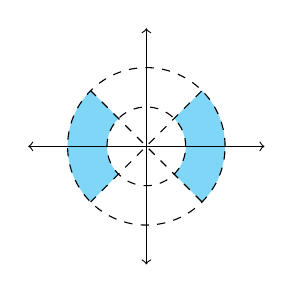
\begin{tikzpicture}

%Esta instrucción colorea arcos "gorditos" de circunferencia
\fill[cyan!50] (45:.5) arc[start angle=45, end angle=-45, radius=.5] -- (-45:1)
	arc[start angle=-45, end angle=45, radius=1] -- cycle;
\fill[cyan!50] (135:.5) arc[start angle=135, end angle=225, radius=.5] -- (225:1)
	arc[start angle=225, end angle=135, radius=1] -- cycle;


\draw[to-to] (1.5,0) -- (-1.5,0);
\draw[to-to] (0,1.5) -- (0,-1.5);

\draw[dashed] (0,0) circle (1 cm) circle (.5 cm);

%Scope y clip cortarán las rectas donde se acaben las circunferencias
\clip (0,0) circle (1 cm);
\draw[dashed] (1,1) -- (-1,-1);
\draw[dashed] (1,-1) -- (-1,1);


\end{tikzpicture}
}